\documentclass{article}

% required 
\usepackage[hyphens]{url} % this wraps my URL versus letting it spill across the page, a bad habit LaTeX has
\usepackage{Sweave}
\usepackage{graphicx}
\usepackage{natbib}
\usepackage{amsmath}
\usepackage{textcomp}%among other things, it allows degrees C to be added
\usepackage{float}
\usepackage[utf8]{inputenc} % allow funny letters in citations 
\usepackage[nottoc]{tocbibind} %should add Re fences to the table of contents?
\usepackage{amsmath} % making nice equations 
\usepackage{listings} % add in stan code
\usepackage{xcolor}
\usepackage{capt-of}%allows me to set a caption for code in appendix 
\usepackage[export]{adjustbox} % adding a box around a map
\usepackage{lineno}
\linenumbers
% recommended! Uncomment the below line and change the path for your computer!
% \SweaveOpts{prefix.string=/Users/Lizzie/Documents/git/teaching/demoSweave/Fig.s/demoFig, eps=FALSE} 
%put your Fig.s in one place! Also, note that here 'Fig.s' is the folder and 'demoFig' is what each 
% Fig. produced will be titled plus its number or label (e.g., demoFig-nqpbetter.pdf')
% make your captioning look better
\usepackage[small]{caption}

\usepackage{xr-hyper} %refer to Fig.s in another document
\usepackage{hyperref}

\setlength{\captionmargin}{30pt}
\setlength{\abovecaptionskip}{0pt}
\setlength{\belowcaptionskip}{10pt}

% optional: muck with spacing
\topmargin -1.5cm        
\oddsidemargin 0.5cm   
\evensidemargin 0.5cm  % same as odd side margin but for left-hand pages
\textwidth 15.59cm
\textheight 21.94cm 
% \renewcommand{\baselinestretch}{1.5} % 1.5 lines between lines
\parindent 0pt		  % sets leading space for paragraphs
% optional: cute, fancy headers
\usepackage{fancyhdr}
\pagestyle{fancy}
%\fancyhead[LO]{Frederik Baumgarten}
%\fancyhead[RO]{Research Proposal}
% more optionals! %
\usepackage{booktabs} %clean and professional look for tables

\graphicspath{ {/Users/frederik/github/PhaenoFlex_clean/analysis/output/} }% tell latex where to find figures 

\begin{document}
	\renewcommand{\bibname}{References}%names reference list 
	
	
	%	\title{
		%	} 
	
	
	\date{\today}
	
	\section*{Aim}
	As climate continues to warm, ecosystems are facing more extreme heat and drought waves. At the same time the potential growing season of temperate and boreal latitudes extends. To which degree plants and forests adapt and indeed prolong their photosynthetic activity in spring and autumn is currently under heavy debate. Not only may soil moisture resources limit plant activity and overall performance but also internal growth control mechanisms could limit further Carbon uptake from the atmosphere. Therefore, this experimental study aimed to provide evidence how longer climatic growing seasons translate into increased biomass production in relation to the negative impacts of drought and heat events. 
	
	\section*{Methods}
	\subsection*{Study species and study site}
	3 year-old saplings of 6 species, each representing a different family were selected to get a wide range of possible tree responses including coniferous evergreen and broad leaved deciduous species. All species selected occur naturally along the Pacific west coast of USA and Canada. The studied deciduous trees were Prunus virginiana L., Acer macrophyllum Pursh., Betula papyfera Marsh. and Quercus garryana Dougl.; evergreen trees were Pinus contorta Dougl., and Sequoia sempervirens (D. Don) Endl. In the following we refer to their genus name only.
	
			\begin{table}[H]
		\centering
		\caption{Species information}
		\begin{tabular}{p{5.8cm} p{2cm} p{2.0cm} p{1.0cm} p{3cm}}
			\toprule
			\textbf{Species name} & \textbf{Family} & \textbf{Initial height} & \textbf{drought tolerance} & \textbf{remarks} \\
			\midrule
			\textit{Prunus virginiana L.} & Rosaceae & x & x &  x  \\
			\textit{Acer macrophyllum Pursh.} & Sapindaceae & x & x & x \\
			\textit{Betula papyfera Marsh.} & Betulaceae &x & x & x \\
			\textit{Quercus garryana Dougl.} & Fagaceae & x & x & x \\
			\textit{Pinus contorta Dougl.} & Pinaceae & x & x &  x\\
			\textit{Sequoia sempervirens (D. Don) Endl.} & Cupressaceae & x & x & x \\
			
			\bottomrule
		\end{tabular}
	\end{table}
	
	The study was conducted on the campus of the University of British Columbia (Totem Field; 49.2572 N, -123.2503 E) located in Vancouver, Canada. The climate is oceanic characterized by the proximity of the Pacific with a mean annual temperature around 10°C (18°C in July and 4°C in January). Together with an annual precipitation of c. 1500mm this climate supports a typical temperate rain forest along the west coast.
	
	\subsection*{Experimental setup}
		
	Saplings arrived in Winter 2023 and were, still dormant, repotted using a medium for perennials consisting of 50\% peat, 25\% crushed pumice and 25\% crushed bark (www.westcreekfarm.com). The low water-retention capacity of this potting medium allowed to accelerate and intensify the effects of the drought treatments. Soil volume was adjusted for each species, specifically doubled in volume compared to the previous container to minimize limitations later in the season (final pot volume: 4.5l for Sequoia and Pinus; 9l for Quercus and Betula; 18l for Acer and Prunus). \\ 
	After potting, saplings received 2g of slow-release NPK fertilizer (osmocote plus) to meet natural conditions. \\ 
	On 31 March 2023, saplings were transferred to cooling chambers set at 4°C with ambient photoperiod conditions to prolong dormancy for one month (until 30 April 2023). The only exception was the saplings designated for growing season extension, which remained at the experimental site. \\ 
	Saplings were then arranged in three blocks, each containing a subset of all treatments. Two blocks were sheltered from rain by an open-walled and well ventilated polytunnel greenhouse to protect sensitive electronics. All saplings were attached to a drip irrigation system (40 PVC frame from Netafilm with a Toro controler) that ensured saturated soil moisture conditions throughout the experiment (120±6 ml water every 6 hours;  except for the drought treatment duration). \\ 
	
		\subsection*{Study design and treatments}
	The whole study design is depicted in Fig. \ref{fig:fig_1xxx} for an overview. Saplings were subjected to a) a growing season extension, b) one out of 3 drought timings, c) one out of 3 defoliation events and d) a heat event, resulting in eight treatments plus control. 15 replicates were randomly assigned to each treatment (8 treatments plus control à 15 replicates = 135 saplings/species). \\  
	
	\textit{Growing season extension} \\
	Growing season extension were achieved by prolonging dormancy of all other treatments for a month (see above). This resulted in an acculuation of xxx growing degree days (GDD) that advanced budburst by X to Y days (depending on species, see XX).\\
	
	\textit{Drought treatments} \\
	Drought treatments were conducted in climate chambers (TPC-19, Biochambers; Canada) at close proximity to the experimental site (Faculty of Forestry, UBC). Drought conditions were simulated with temperatures set to 30°C during the day and 20°C at night. These temperatures rose and fell at the same time every day, corresponding to the photoperiod at Vancouver’s summer solstice (i.e. photoperiod: 16h and 15min). The photoperiod was adjusted weekly, to the current ambient sunrise and sunset time. 
	The first drought treatment started species-specific once leaf-out reached stage 4 (i.e. leaves fully unfolded). Second and third drought treatment were started on a fixed date, namely 23 June and 31 July 2023. Subsequent drying of the pots was monitored by measuring whole pot weight (balance accuracy 0.1g) as well as volumetric water content (VWC, Fieldscout TDR 150). Saplings were released from drought stress on species-specific dates, marked by the first signs of desiccation, such as curled or discolored leaves, and soil moisture levels approaching the wilting point. %for several days...curves? or even argue with poor recovery during the night of stem diameter 
	Saplings were again weighted under field capacity and then transferred back to the experimental site and plugged into the irrigation system. \\
	
	\textit{Defoliation treatments} \\
	The defoliation treatments were intended to simulate leaf loss due to frost, browsing, hail or overheating. As these scenarios cause different physiological reactions (e.g. release of defence substances), we cut off each fully unfolded leaf (stage 4) halfway up the petiole using pruning scissors. Younger stages were left intact to prevent accidental damage to the meristem. The leaf area was reduced to 0\% for all deciduous species. For pines, all needles older than 1 year were removed by hand by tearing them delicately in the direction of the apex. The current year needles were preserved in the first defoliation treatment since they were less than 1cm in length and still developing. In the second and third defoliation event c. ¾ of the current-year needles were removed, which presumably contributed already most to the total photosynthetic assimilation. All defoliation events coincided with the start of the respective drought treatments, i.e. the first defoliation took place on the same day as the start of the first drought treatment. In the following two weeks we continuously cut all newly emerging leaves reaching stage 4 to suspend all assimilate supply. %mention here the weight of the leaves	All the leaves collected were gathered in brown paper bags, where all the replicates from the same species were put together to dry. The leaves were dried for 48 hours at 70°C in a drying oven (VWR 1645D). Dry matter biomass was measured with scale (Scout Pro) to an accuracy of two decimal places (0.00 grams).
	Subsequent recovery of saplings was assessed by eye as the percentage of recovering leaf area compared to a control sapling. 
	
	
	
	
		\begin{figure}[H]
		\centering
		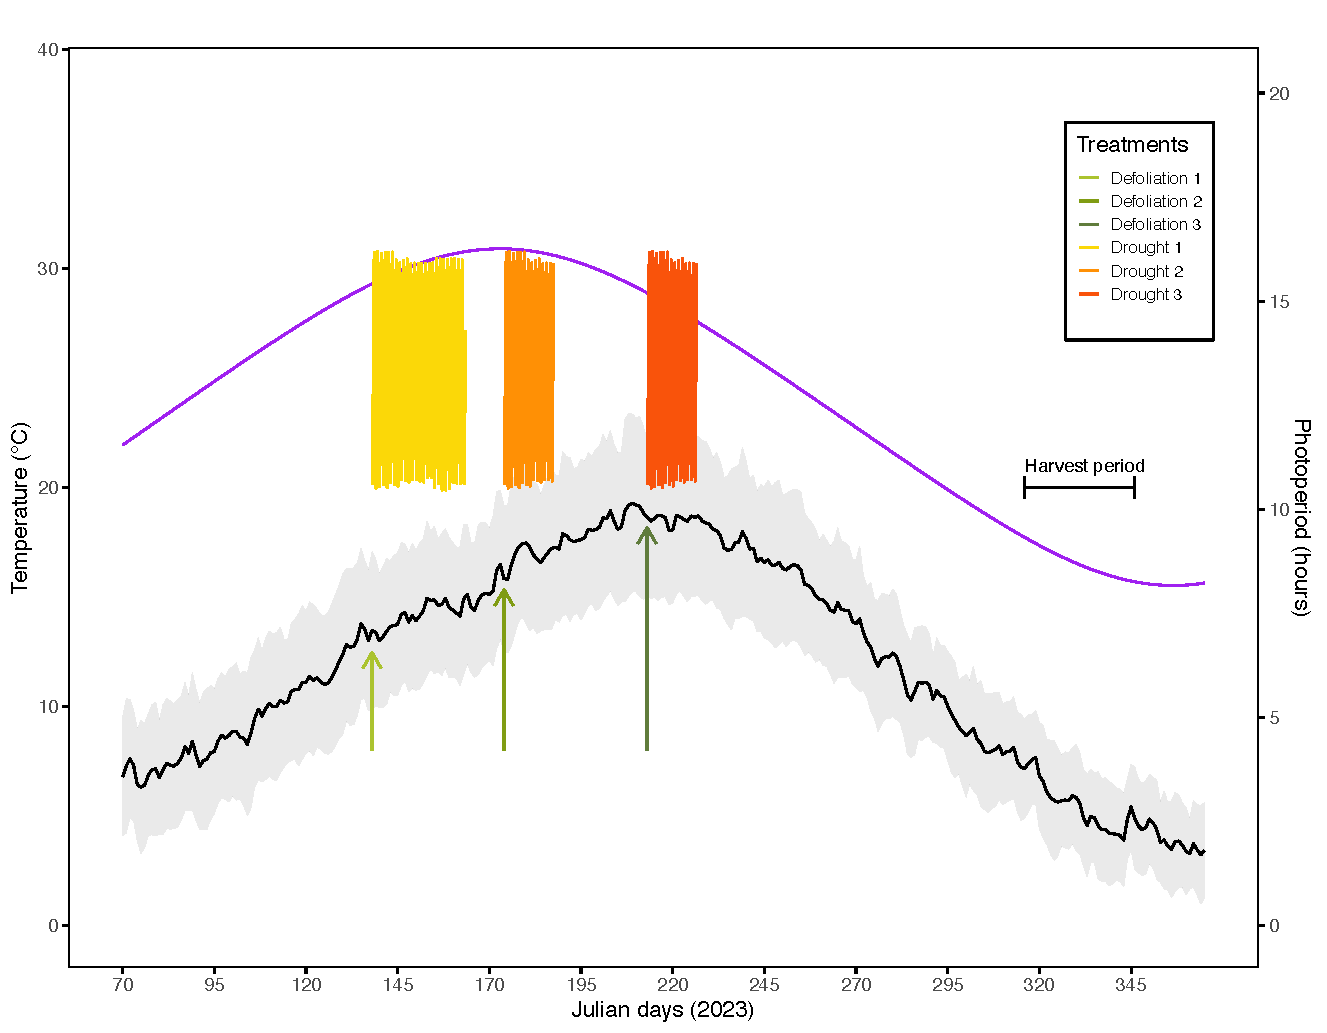
\includegraphics[width=0.9\textwidth]{design.pdf} 
		\caption{Effect size in g of biomass compared to control sapling when exposed to an extended growing season (GS\_extend), heat, defoliation or drought event. Colors represent the six study species. }
		\label{fig:fig_1xxx}
	\end{figure}
	
	\subsection*{Phenological monitoring}
		\textit{Leaf emergence} \\
	Bud development in spring was assessed by the same observer twice a week starting 24 April 2023 using a categorical scale depending on species. Deciduous species were scored on a four-stage scale (see \citep{vitasseElevationalAdaptationPlasticity2013a}): stage 0 - dormant, stage 1 - bud swelling, stage 2 - bud burst, stage 3 - leaf-out and stage 4 - leaf unfolded. Pine saplings were scored differently as follows: stage 1 - swelling or elongation of shoot visible, stage 2 - green needle tips along the shoot visible, stage 3 - scales open along the shoot and first needles become visible, stage 4 - green needles emerging away from the shoot. Phenostages for Sequoia were limited to two stages because this species does not form buds: stage 1 - first signs of needles visible at the apical meristem but all bended inwards towards the center, stage 2 - needles start to grow and bend outwards from the center.
	For all species and saplings the day of year was recorded as soon as 50\% of all buds reached the newest stage. \\
	
		\textit{Bud set} \\
		Cessation of bud development was monitored starting in early July 2023 until the apical bud was dormant. Bud set was generally scored on a four-stage score as follows: stage 3 - ongoing shoot growth/elongation, stage 2 - apical bud forms and remains as a light-green bud with the last (pair) of leaves remaining small, stage 1 - first bud scales appear, stage 0 - bud turns dark red/brown and hardens. In Acer only stages 3, 2 and 0 were distinguished and recorded. Bud set of Pinus and Sequoia were not monitored, since shoot elongation was the best activity proxy of the shoot apical meristem.\\
		
		\textit{Leaf senescence} \\
		Leaf senescence was monitored in weekly intervals between 1 Sept 2023 and 4 Nov 2023 i.e. until all leaves were shed. For each sapling and at every monitoring occasion the chlorophyll content was estimated using a leaf spectral index (LSI; mean of three representative leaves per replicate; MC-100, apogee instruments). Following  \citep{zohner} this value was weighted by simultaneous estimates of the percentage of remaining green leaves (by eye; 100\%=all leaves remaining; 0\%=all leaves shed). For example, a sapling with 50\% remaining leaves and a mean LSI of 10 was rated with a total LSI of 10 (0.5 * 20). A sapling was considered senescent one a value was below 50\% of the maximum LSI value. \\
		%In addition, light curves, Amax measurements
		
		
		
			
\begin{table}[H]
	\captionsetup{justification=raggedright, singlelinecheck=false} % Left-align caption
	\centering
	\caption{Phenological stages used for all deciduous species \citep{vitasseElevationalAdaptationPlasticity2013a}, pine as well as Sequoia}
	\begin{tabular}{p{2.4cm} p{1cm} p{2.5cm} p{8.0cm}} % Make sure the formatting is correct
		\toprule
		\textbf{Group} & \textbf{Scale} & \textbf{Phenostage} & \textbf{Description} \\
		\midrule
		
		\multicolumn{4}{l}{\textit{Deciduous species}} \\
		& 0 & dormant & no bud development visible \\
		& 1 & bud swelling & swollen and/or elongating buds \\
		& 2 & budburst & bud scales open and leaves partially visible \\
		& 3 & leaf-out & leaves fully emerged from bud but still folded, crinkled or pendant \\
		& 4 & leaf unfolding & leaves fully unfolded \\
		\midrule
		
		\multicolumn{4}{l}{\textit{Pine}} \\
		& 0 & dormant & no signs of activity \\
		& 1 & swelling & swelling or elongation of shoot visible \\
		& 2 & budburst & green needle tips along the shoot visible \\
		& 3 & leaf-out & scales open along the shoot and first needles become visible \\
		& 4 & leaf-unfolding & green needles emerging away from the shoot \\
		\midrule
		
		\multicolumn{4}{l}{\textit{Sequoia}} \\
		& 1 & not active & first signs of needles visible at the apical meristem but all bent inwards towards the center \\
		& 2 & active & needles start to grow and bend outwards from the center \\
		\bottomrule
	\end{tabular}
\end{table}


			
	\subsection*{Soil moisture measurements}
Everyday, at the same time, the volumetric water content (VWC) was measured using a soil moisture meter (Fieldscout TDR 150). The rod length was changed depending on the pot depth that varied for different species (i.e. …). One was 12.2 cm and the other was 20.32 cm. In addition, and for a more integrated indicator of soil water loss especially near the wilting point, whole pots were weighted using a scale (REF) to an accuracy of 1g. To avoid noise in the radial monitoring data, replicates equipped with magnetic dendrometers were only weighted at the start and end of the drought treatments. %Since VWC and weight loss yielded a strong correlation (Fig SX) whole VWC curves were calculated also for these replicates.\\

	\subsection*{Shoot apical growth}
	Shoot growth activity of the apical meristem was measured on 10 replicates per treatment throughout the season in biweekly intervals. Water resistant measuring tapes were attached to the stem base under the terminal bud after budburst and subsequent shoot elongation was tracked on the tape.  \\

	\subsection*{Radial growth and tree-water deficit}
To track radial growth, magnetic dendrometers were installed that were designed to not injure the bark during installation and operate without friction \citep{clonchHighPrecisionZerofriction2021}. Devices were installed at the stem base avoiding branches and abnormalities using breathable bandage material (). Five control replicates were equipped permanently while drought treatments swiched devices so that five replicates of every drought timing captured diameter fluctuations 1 week prior, during and 2 weeks after the respective drought treatment. \\

	\subsection*{Biomass assessment}
	Before budburst and after the growing season we measured diameter c. 2 cm above plant collar (digital calliper; accuracy ±0.1mm) and height (graduated pole; accuracy ±1mm) of each sapling. Total above-ground biomass was estimated following allometric equations provided by \citet{annighoferSpeciesspecificGenericBiomass2016}. Substracting before from after season estimates revealed the calculated above-ground biomass increment.	\\
After entering full dormancy, all saplings were removed from pots in December 2023 to wash off the potting substrate. Whole saplings where dried at 80° C for 48h before tissue was separated into roots and shoots with the latter being further sorted into current year and past years tissue. All partial quantities were weighted with an accuracy of ±0.01g.\\

	\subsection*{Wood anatomy}
Prior to every drought and defoliation event, 10 replicates were pinned at a homogenous stem section at the base using a needle and dyed with ethylene blue \citep{gartnerCambialActivityMoringa2021a}. This pinning hole acted as a `marker in time' that allowed to separate wood formation before and after treatment start. During harvest at the end of the growing season, a 2cm section containing the pinning hole was cut using an electric saw and stored in 35\% ethanol solution. \\
C. four stem sections per replicate were cut using a microtome (semi-automated Lab-microtome, WSL; thickness: 15\textmu m) to ensure the visiblilty of the anatomical structure around the pinning hole. Sections were double stained with Safranin (to color lignified structures red) and Astrablue (to color unlignified structures blue) following standard protocol \citep{gartnerMicroscopicPreparationTechniques2013}. Sampled where then fixed using UV-sensitive mounting medium (Eukitt UV, Fisher scientific) and dried under a commercial nail dryer UV-lamp for c. two minutes. Samples where then scanned with a slide scanner () and then processed with xxxx.

	\subsection*{Data analysis and statistics}
	
	
	\section*{Preliminary results}
	
	
	\begin{figure}
	\centering
	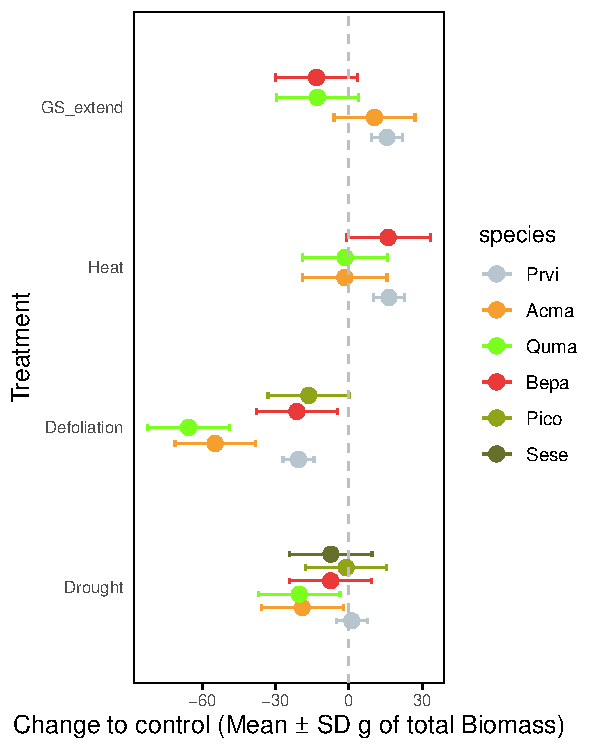
\includegraphics[width=0.9\textwidth]{posteriors/biomass_post_solst_treat_sub.pdf} 
	\caption{Effect size in g of biomass compared to control sapling when exposed to an extended growing season (GS\_extend), heat, defoliation or drought event. Colors represent the six study species. }
	\label{fig:fig_1xxx}
\end{figure}
	
	
			\begin{figure}
		\centering
		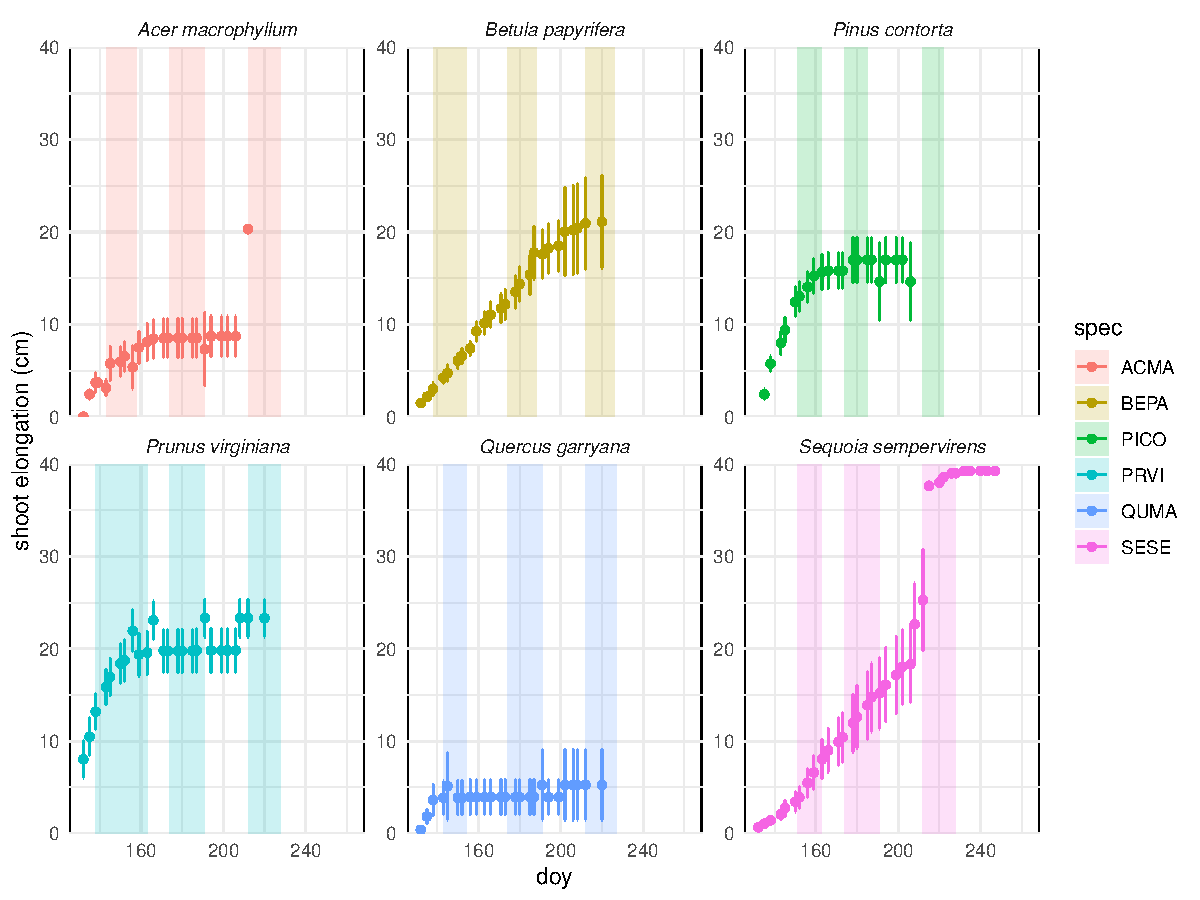
\includegraphics[width=0.9\textwidth]{shoot_elongation copy.pdf} 
		\caption{Shoot extension over the growing season 2023 for the six study species. Note the species-specific differences in absolute growth and in growth phenology with Quercus stopping first and Sequoia elongating until the very end of the season.}
		\label{fig:fig_1xxx}
	\end{figure}
	
	
				\begin{figure}
		\centering
		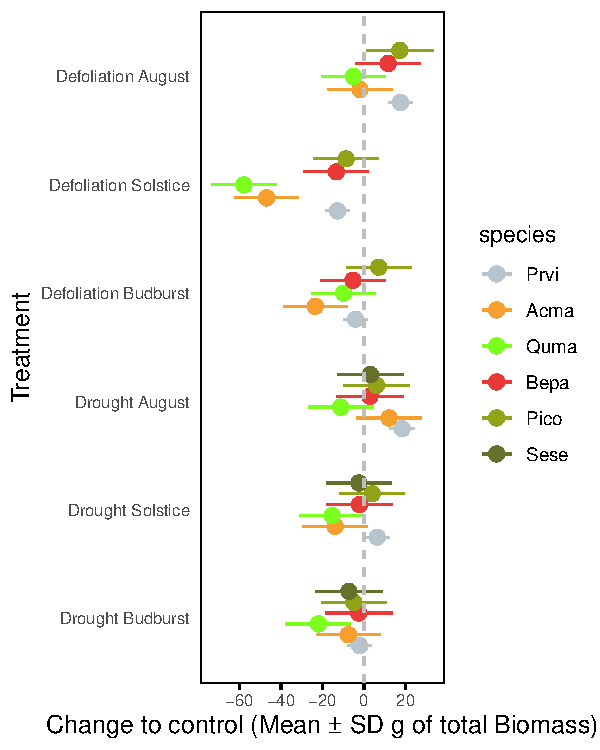
\includegraphics[width=0.9\textwidth]{posteriors/biomass_post_treat_sub.pdf} 
		\caption{Effect size in g of biomass compared to control sapling when exposed to defoliation or drought treatments on 3 occasions. Colors represent the six study species.}
		\label{fig:fig_1xxx}
	\end{figure}
	
	
	
	
	\begin{table}[h!]
		\begin{center}
			\caption{Details of saplings origin }
			\label{tab:table1}
			\begin{tabular}{l|c|r} % 
				\textbf{Species} & \textbf{Nursery} & \textbf{Seed origin}\\
				%$\alpha$ & $\beta$ & $\gamma$ \\
				\hline
				Prunus virginiana L. & Peel's Nurseries Ltd. & BC Canada\\
				Acer macrophyllum Pursh. & Streamside Native Plants & BC Canada\\
				Betula papyfera Marsh. & Peel's Nurseries Ltd. &BC Canadac\\
				Quercus garryana ?.& Peel's Nurseries Ltd. & BC Canada\\
				Populus trichocarpa Torr. & Peel's Nurseries Ltd.& BC Canada\\
				Pinus contorta, Dougl. & Tree Time Services Inc & Alberta Canada\\
				Sequoia sempervirens(D. Don)&? & California\\
				
			\end{tabular}
		\end{center}
	\end{table}
	
	\subsection*{Drought treatments}
	//move here the general timings and explanations as this is the main treatment//
	
	Dendrometer installation //could you provide information on the software, location where they were build, etc.// 
	Once all the trees were in their respective blocks and drip irrigation installed, we set up the dendrometers on the control replicates and the first drought treatment replicates. 
	//reminder: tape //
	
	Swiss dendrometers
	//update this section//
	
	Climate chambers temperature and humidity
	We set the climate chambers to identical conditions for all drought treatments. The night temperature was set at 20 °C and the day temperature was set to 30 °C. These temperatures rose and fell at the same time every day, which corresponds to the time of sunrise and sunset at Vancouver’s summer solstice (i.e. 16h and 15min). The photoperiod was adjusted weekly, to the current ambient sunrise and sunset time. Hence. Four climate chambers from *** and one walk in chamber from *** were used and all of them are located in UBC’S Faculty of Forestry’s basement. For the first drought treatment dehumidifiers (Toshiba TDDP2213ES2) were set in the climate chambers at a set humidity of 35%, in order to avoid relative humidity differences that could affect the tree’s transpiration rate //should we add the date at which they were added?//. Indeed, if one growth chamber has a higher relative humidity than another, the plants in this one would reach the wilting point later than the others. 
	
	Dro 1 start decision:
	The first drought treatment started species-specific once leaf-out reached stage 4 (i.e. leaves fully unfolded). Specifically, the plants were moved to climate chambers () where they experienced 30 °C. during the day and 20 °C. during the night. While temperature cycles were constant across all four drought treatments to ensure comparability, the photoperiod followed ambient conditions, between treatments The trees were left to dry in the chambers for different periods depending on the species. For the first drought treatment, we removed the trees once one replicate from a species showed drought stress morphological symptoms. We assumed that at least one replicate reached their species’ wilting point. The removal decision was made on a species-specific basis and was arbitrary, as we observed distinct variations in the speed of symptom manifestation and their severity among individuals within the replicates of a single species. To avoid high mortality rate, we decided to remove all the replicates once one showed severe desiccation symptoms. The trees were then removed from the climate chambers, saturated with water, and reintroduced in the field, where they were reconnected to the irrigation system. Dendrometers were kept on these replicates for a minimum period of two weeks to monitor radial growth following this drought treatment. After this, the dendrometers were placed on the second drought treatment replicates for 5 to 7 days which allowed us to monitor radial growth prior to their shift in the climate chambers.
	
	Dro 2, 3, 4 start decision
	The replicates selected for the following drought treatments were all moved at the same time. The decision of removal for the second drought treatment was slightly different. Since we had access to the rate of water loss and the VWC at which the replicates from the first drought treatment reached their wilting point, we included these factors in the decision process. // Should we mention the decision steps we discussed. Would a simple figure be a good idea for this // Once all the replicates were removed from the climate chambers, they stayed in the field for two weeks for radial monitoring, then the dendrometers were set for the following drought treatment //(idem for dro1, 2, 3, 4, how could we avoid repetition?//
	
	
	\subsection*{Defoliation treatments}
	Two defoliation treatments were applied at the same time during the summer, one that started on May 16th, and the second, on June 23rd. Those treatments were designed to mimic a net loss of leaf area induced by either browsing, spring frost or drought. 
	
	Timing:
	•	We conducted the first defoliation treatment once the leaves from most of the replicates of one species have reached the fourth phenological stage. This stage was reached at different times, depending on the species, therefore, the start of this treatment was species-specific. 
	•	The second defoliation treatment was conducted after the theoretical peak growth period that happens around summer solstice. At that time, all species have reached the fourth phenological stage. 
	
	Defoliation:
	Deciduous trees 
	Using pruning snips (Fiskars Garden), we cut all the leaves mid petiole that were at phenological stage 4. We selected this technique which was in several studies (Miller Tworkoski, 2010; Nzima, Martin, Nishijima, 1999).Younger stages were left intact to not accidentally damage the terminal meristem. In the following two weeks we continuously cut all newly emerging leaves reaching stage 4 to suspend all assimilate supply.
	
	Evergreen (Pinus)
	All one-year-old and older mature needles were removed by hand by tearing them delicately in the direction of the apex to not hurt the bark as mentioned in (O’Neil, 2011). The current year needles were preserved in the first defoliation treatment since they were less than 1cm in length and still developing. In the second treatment we additionally defoliated c. ¾ of the current-year needles which were still not fully elongated but presumably contributed already most to the total photosynthetic assimilation.
	//I think we should mention here the weight of the leaves we removed. Perhaps we make a table out of that. //
	
	Drying:
	All the leaves collected were gathered in brown paper bags, where all the replicates from the same species were put together to dry. The leaves were dried for 48 hours at 70°C in a drying oven (VWR 1645D). Dry matter biomass was measured with scale (Scout Pro) to an accuracy of two decimal places (0.00 grams).
	
	\subsection*{Soil moisture measurements}
	Everyday, at the same time, the volumetric water content (VWC) was measured using a soil moisture meter (Fieldscout TDR 150). The rod length was changed depending on the pot depth that varied for different species (i.e. …). One was 12.2 cm and the other was 20.32 cm. In addition, and for a more integrated indicator of soil water loss especially near the wilting point, whole pots were weighted using a scale (REF) to an accuracy of 1 gram. To avoid noise in the radial monitoring data, replicates equipped with magnetic dendrometers were only weighted at the start and end of the drought treatments. Since VWC and weight loss yielded a strong correlation (Fig SX) whole VWC curves were calculated also for these replicates.
	
	
	
	
	
	\begin{figure}
		\centering
		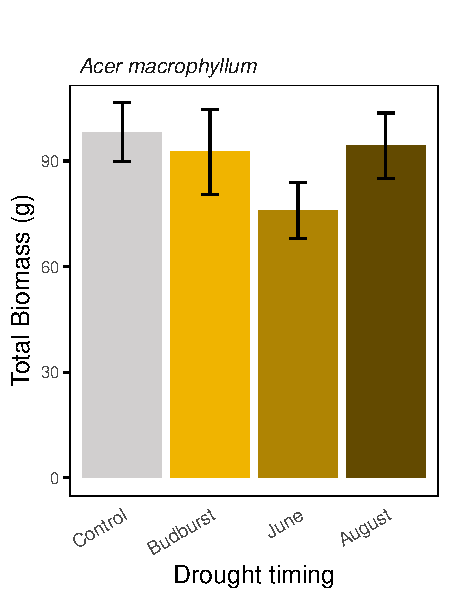
\includegraphics[width=0.9\textwidth]{biomass_tot_Acma.pdf} 
		\caption{xxxxxxxxxxx}
		\label{fig:fig_1xxx}
	\end{figure}
	
	
	
	\section*{stuff I did't find place yet}
	
	
	\newpage
	
	
	\bibliography{refs_PhaenFlex}
	\bibliographystyle{ecolett}
	
	
	
	
	
	
\end{document}
